\documentclass{beamer}

% Packages
\usepackage{amsmath}
\usepackage{graphicx}
\usepackage{tikz}
\usepackage{multicol}

\title{9.ex.5}
\author{EE24BTECH11036 - Krishna Patil}
\date{}

\begin{document}

\begin{frame}
\titlepage
\end{frame}

\begin{frame}
\frametitle{Question}
\textbf{Question:} Verify that the function \( y = a \cos{x} + b \sin{x} \), where \( a, b \in \mathbb{R} \), is a solution of the differential equation 
\[
\frac{d^2y}{dx^2} + y = 0 
\]
if \( y(0) = a \) and \( y'(0) = b \).
\end{frame}

\begin{frame}
\frametitle{Theoretical Solution}
The given differential equation is a second-order linear ordinary differential equation.

Let \( y(0) = a \) and \( y'(0) = b \).

By the definition of Laplace transform:
\[
\mathcal{L}\left(f(t)\right) = \int_0^{\infty} e^{-st} f(t) \, dt
\]
Some important properties of Laplace transform:
\begin{align*}
    \mathcal{L}\left(y''\right) &= s^2 \mathcal{L}\left(y\right) - s y(0) - y'(0) = s^2 \mathcal{L}\left(y\right) - sa - b \\
    \mathcal{L}\left(\cos{t}\right) &= \frac{s}{s^2 + 1} \\
    \mathcal{L}\left(\sin{t}\right) &= \frac{1}{s^2 + 1}
\end{align*}
\end{frame}

\begin{frame}
\frametitle{Laplace Transform of the Differential Equation}
Applying the Laplace transform on the given differential equation:
\[
y'' + y = 0
\]
we get:
\[
\mathcal{L}\left(y''\right) + \mathcal{L}\left(y\right) = 0
\]
\[
s^2 \mathcal{L}\left(y\right) - sa - b + \mathcal{L}\left(y\right) = 0
\]
\[
\mathcal{L}\left(y\right) = \frac{sa + b}{s^2 + 1} = a\frac{s}{s^2 + 1} + b\frac{1}{s^2 + 1}
\]
Taking the inverse Laplace transform:
\[
y = a \mathcal{L}^{-1}\left(\frac{s}{s^2 + 1}\right) + b \mathcal{L}^{-1}\left(\frac{1}{s^2 + 1}\right)
\]
\[
y = a \cos{x} + b \sin{x}
\]
Thus, the function \( y = a \cos{x} + b \sin{x} \) is indeed a solution to the differential equation.
\end{frame}

\begin{frame}
\frametitle{Computational Solution: Trapezoidal Method}
The given differential equation can be represented as:
\[
y'' + y = 0
\]
Let \( y = y_1 \) and \( y' = y_2 \), then:
\[
\frac{dy_2}{dx} = -y_1 \quad \text{and} \quad \frac{dy_1}{dx} = y_2
\]
Discretizing the steps using the Trapezoid rule:
\[
y_{2, n + 1} - y_{2, n} = -\frac{h}{2}(y_{1, n} + y_{1, n + 1})
\]
\[
y_{1, n + 1} - y_{1, n} = \frac{h}{2}(y_{2, n} + y_{2, n + 1})
\]
Solving for \( y_{1, n + 1} \) and \( y_{2, n + 1} \):
\[
y_{1, n + 1} = \frac{(4 - h^2) y_{1, n} + 4 h y_{2, n}}{(4 + h^2)}
\]
\[
y_{2, n + 1} = \frac{(4 - h^2) y_{2, n} - 4 h y_{1, n}}{(4 + h^2)}
\]
\end{frame}

\begin{frame}
\frametitle{Computational Solution: Bilinear Transform}
We apply the Laplace transform:
\[
Y(s) = \frac{sa + b}{s^2 + 1}
\]
Using the Bilinear transform:
\[
s = \frac{2}{h} \frac{1 - z^{-1}}{1 + z^{-1}}
\]
\[
Y(z) = \frac{2 h a (z^2 - 1) + b h^2 (z + 1)^2}{(h^2 + 4) z^2 + 2 (h^2 - 4) z + (h^2 + 4)}
\]
Rewriting this, we get the difference equation:
\[
\boxed{
z^2 Y(z) + 2 \frac{h^2 - 4}{h^2 + 4} z Y(z) + Y(z) = \frac{(2 h a + b h^2) z^2 + (2 h^2 b) z + (h^2 b - 2 h a)}{h^2 + 4}
}
\]
By taking the inverse \( z \)-transform, we obtain the difference equation:
\[
\boxed{
y_{n + 2} + 2 \frac{h^2 - 4}{h^2 + 4} y_{n + 1} + y_n = \frac{(h^2 b - 2 h a - y_0)}{h^2 + 4}
}
\]
\end{frame}

\begin{frame}
\frametitle{Region of Convergence (ROC)}

\begin{block}{\textbf{Laplace Transform ROC:}}
\[
\boxed{\text{Re}(s) > 0}
\]
The ROC is the right half of the complex plane.

\end{block}

\vspace{0.5cm}

\begin{block}{\textbf{Bilinear Transform ROC:}}
\[
\boxed{|z| < 1}
\]
The ROC is the inside of the unit circle in the Z-plane.
\end{block}

\end{frame}

\begin{frame}
\frametitle{Results: Plot Comparison}
Iteratively solving the difference equations and plotting the results using the Trapezoidal method and Bilinear transform, we get the following plot:

\begin{figure}[h!]
    \centering
    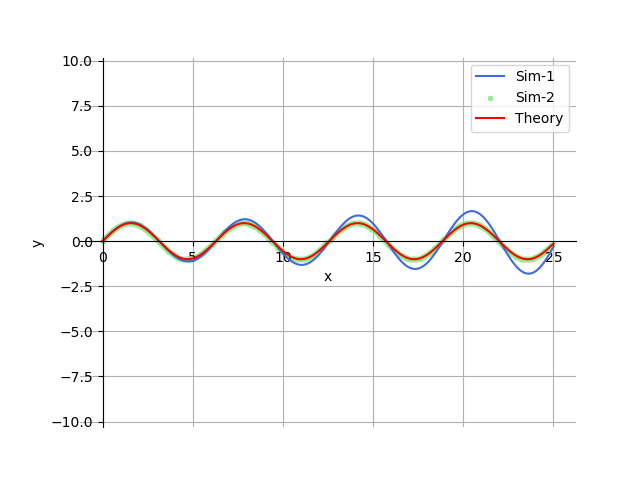
\includegraphics[width=0.7\columnwidth]{figs/graph.png}
    \caption{Sim-1 is from the Trapezoidal Method and Sim-2 is from the Bilinear Transform, showing the accuracy of the Bilinear method.}
\end{figure}

\end{frame}

\end{document}

